\newpage
\section{Lecture-13}
\subsection{Double Integrals}
\begin{definition}
    Assume $D\subseteq\mathbb R^2$ is bounded, and let $f(x,y)$ be bounded on $D$. Let $A$ be a rectangle containing $D$, and define $$\Tilde{f}(x,y)=\begin{cases}
        f(x,y), & (x,y)\in D\\
        0, & (x,y)\in A\setminus D
    \end{cases}$$
    then we redefine, 
    $$
    \iint_D f(x,y)dxdy=\iint_A \Tilde{f}(x,y)dxdy 
    $$
\end{definition}
Properties of double integrals:
\begin{enumerate}
    \item if $f(x,y)$ is continuous on $D$ then the integral $\iint_D f(x,y)dxdy$ exists.
    \item if $f(x,y)$ is ``almost" continuous then $f$ is integrable on $D$.
    \item (Linearity) Assume $f,g$ are integrable on $D$, 
    $$\iint_{D}\alpha f+\beta g=\alpha\iint_{D}f+\beta \iint_{D}g$$
    \item (Monotonicity) If $f\leq g$ then
    $$\iint_{D} f\leq \iint_{D} g$$
    \item No formula for $\iint_{D} fg$
    \item If $|f|$ is integrable and $$\left|\iint_{D}f\right|\leq \iint_{D}|f|$$
    \item $$m\operatorname{Area}(D)\leq\iint_{D} f\leq M\operatorname{Area}(D)$$
    \item if $f$ is continuous on $D$, and $D$ is connected then $$\iint_{D} f(x,y)dxdy=f(x_0,y_0)\operatorname{Area}(D)$$ 
    \begin{proof}
    $$m\leq\frac{\iint_{D} f}{\operatorname{Area}(D)}\leq M\stackrel{IVT}{\implies} \exists (x_0,y_0)\in D:f(x_0,y_0)=\frac{\iint_{D} f}{\operatorname{Area}(D)}$$
    \end{proof}
    \item (Additivity) if $D=D_1\cup D_2$ and $D_1\cap D_2=\emptyset$ or $D_1\cap D_2$ is of $0$ area, t hen, 
    $$
    \iint_{D} f=\iint_{D_1} f+\iint_{D_2} f
    $$
\end{enumerate}
\begin{theorem}
If \(f(x,y)\) is continuous on
\[
D=[a,b]\times[c,d],
\]
then
\[
\iint_D f(x,y)\,dA
=
\int_a^b \int_c^d f(x,y)\,dy\,dx
=
\int_c^d \int_a^b f(x,y)\,dx\,dy.
\]
These integrals are called \emph{iterated integrals}.
\end{theorem}
\begin{example}
    $f(x,y)=xy$ where $D=[1,2]\times\left[\frac\pi4,\frac\pi3\right]$
    \begin{align*}
        \iint_D xy dxdy &= \int_1^2 \left(\int_{y=\frac\pi3}^{y=\frac\pi4} xy dy\right)dx\\
        &= \int_1^2 \left( \left.x\frac{y^2}{2}\right|_{y=\frac\pi3}^{y=\frac\pi4}\right)\\
        &= \frac12\left[\left(\frac\pi3\right)^2-\left(\frac\pi4\right)^2\right]\int_1^2 xdx\\
        &= \frac12 \left(\frac{\pi^2}{9}-\frac{\pi^2}{16}\right)\left.\frac{x^2}{2}\right|_1^2
    \end{align*}
\end{example}
\begin{example}
    A standard counterexample (showing that Fubini's theorem can fail when the hypotheses are not satisfied) is the function
\[
f(x,y)=
\begin{cases}
\dfrac{x^2-y^2}{(x^2+y^2)^2}, & (x,y)\ne(0,0),\\[6pt]
0, & (0,0),
\end{cases}
\]
defined on the square \([-1,1]\times[-1,1]\).

This function is not continuous at \((0,0)\).

For fixed \(x\ne 0\),
\[
\int_{-1}^1 f(x,y)\,dy
=
\int_{-1}^1 \frac{x^2-y^2}{(x^2+y^2)^2}\,dy
=
\left[\frac{y}{x^2+y^2}\right]_{-1}^{1}
=
\frac{2}{1+x^2}.
\]
Therefore,
\[
\int_{-1}^1\left(\int_{-1}^1 f(x,y)\,dy\right)dx
=
\int_{-1}^1 \frac{2}{1+x^2}\,dx
=
\pi.
\]

On the other hand, for fixed \(y\ne 0\),
\[
\int_{-1}^1 f(x,y)\,dx
=
\int_{-1}^1 \frac{x^2-y^2}{(x^2+y^2)^2}\,dx
=
\left[-\frac{x}{x^2+y^2}\right]_{-1}^{1}
=
-\frac{2}{1+y^2}.
\]
Hence,
\[
\int_{-1}^1\left(\int_{-1}^1 f(x,y)\,dx\right)dy
=
\int_{-1}^1 -\frac{2}{1+y^2}\,dy
=
-\pi.
\]

Thus,
\[
\int_{-1}^1 \int_{-1}^1 f(x,y)\,dy\,dx = \pi,
\qquad
\int_{-1}^1 \int_{-1}^1 f(x,y)\,dx\,dy = -\pi.
\]

So the two iterated integrals are different.
\end{example}


\begin{center}
\begin{tikzpicture}[scale=1.0, >=Stealth, every node/.style={font=\small}]

% ===================== Case 1 =====================
\begin{scope}[xshift=0cm, yshift=0cm]
    \node at (2.7,5.0) {Case 1};

    % Axes
    \draw[->] (0,0) -- (5.2,0) node[right] {$x$};
    \draw[->] (0,0) -- (0,4.3) node[above] {$y$};

    % Vertical dashed lines
    \draw[dashed] (1,0) -- (1,3.0);
    \draw[dashed] (4.2,0) -- (4.2,2.1);
    \node[below] at (1,0) {$a$};
    \node[below] at (4.2,0) {$b$};

    % Shaded region
    \fill[green!35]
        plot[smooth] coordinates {
            (1,3.0) (1.5,2.8) (2.0,2.9) (2.8,3.9) (3.5,3.3) (4.2,2.1)
        }
        --
        plot[smooth] coordinates {
            (4.2,2.1) (3.6,1.8) (2.8,1.7) (2.0,1.7) (1.4,1.9) (1,2.2)
        }
        -- cycle;

    % Top and bottom curves
    \draw[red, thick]
        plot[smooth] coordinates {
            (1,3.0) (1.5,2.8) (2.0,2.9) (2.8,3.9) (3.5,3.3) (4.2,2.1)
        };

    \draw[blue, thick]
        plot[smooth] coordinates {
            (1,2.2) (1.4,1.9) (2.0,1.7) (2.8,1.7) (3.6,1.8) (4.2,2.1)
        };

    % Labels
    \node at (2.15,3.65) {$y=g_2(x)$};
    \node at (3.1,1.45) {$y=g_1(x)$};
\end{scope}

% ===================== Case 2 =====================
\begin{scope}[xshift=8.0cm, yshift=-0.1cm]
    \node at (1.8,5.0) {Case 2};

    % Axes
    \draw[->] (-0.8,0) -- (3.7,0) node[right] {$x$};
    \draw[->] (0,0) -- (0,4.9) node[above] {$y$};

    % Dashed horizontal lines
    \draw[dashed] (0,4.0) -- (0.75,4.0);
    \draw[dashed] (0,1.0) -- (0.95,1.0);

    % Labels on y-axis
    \node[left] at (0,4.0) {$d$};
    \node[left] at (0,1.5) {$c$};

    % --- Filled region ---
    % Go along left boundary from top to bottom,
    % then bottom segment,
    % then right boundary from bottom to top,
    % then top segment back to the start.
    \fill[green!35]
        plot[smooth] coordinates {
            (0.75,4.0)
            (0.60,3.4)
            (0.55,2.6)
            (0.65,1.8)
            (0.90,1.0)
        }
        --
        (1.75,1.0)
        plot[smooth] coordinates {
            (1.75,1.0)
            (2.35,1.4)
            (2.60,2.3)
            (2.45,3.2)
            (2.05,3.8)
            (1.55,4.0)
        }
        --
        (0.75,4.0)
        -- cycle;

    % Left boundary x = h_1(y)
    \draw[blue, thick]
        plot[smooth] coordinates {
            (0.75,4.0)
            (0.60,3.4)
            (0.55,2.6)
            (0.65,1.8)
            (0.90,1.0)
        };

    % Right boundary x = h_2(y)
    \draw[red, thick]
        plot[smooth] coordinates {
            (1.75,1.0)
            (2.35,1.4)
            (2.60,2.3)
            (2.45,3.2)
            (2.05,3.8)
            (1.55,4.0)
        };

    % Top and bottom boundary segments
    \draw[green!50!black, thick] (0.75,4.0) -- (1.55,4.0);
    \draw[green!50!black, thick] (0.90,1.0) -- (1.75,1.0);

    % Curve labels
    \node at (2.2,3.7) {$x=h_2(y)$};
    \node at (0.95,1.7) {$x=h_1(y)$};
\end{scope}

\end{tikzpicture}
\end{center}

\vspace{0.5em}

We will often use \emph{set builder notation} to describe these regions. Here is
the definition for the region in Case 1:
\[
D=\{(x,y)\mid a\le x\le b,\ g_1(x)\le y\le g_2(x)\}
\]

and here is the definition for the region in Case 2.
\[
D=\{(x,y)\mid h_1(y)\le x\le h_2(y),\ c\le y\le d\}
\]

This notation is really just a fancy way of saying we are going to use all the
points, \((x,y)\), in which both of the coordinates satisfy the two given
inequalities.

The double integral for both of these cases are defined in terms of iterated
integrals as follows.

In Case 1 where \(D=\{(x,y)\mid a\le x\le b,\ g_1(x)\le y\le g_2(x)\}\) the
integral is defined to be,
\[
\iint_D f(x,y)\,dA
=
\int_a^b \int_{g_1(x)}^{g_2(x)} f(x,y)\,dy\,dx
\]

In Case 2 where \(D=\{(x,y)\mid h_1(y)\le x\le h_2(y),\ c\le y\le d\}\) the
integral is defined to be,
\[
\iint_D f(x,y)\,dA
=
\int_c^d \int_{h_1(y)}^{h_2(y)} f(x,y)\,dx\,dy
\]




\begin{example}
Evaluate the double integral
\[
\iint_D (x^3+y^3)\,dx\,dy
\]
where \(D\) is the region bounded by the lines
\[
y=\frac{x}{2}, \qquad y=x, \qquad x=4.
\]

Equivalently, \(D\) is described by
\[
0\le x\le 4, \qquad \frac{x}{2}\le y\le x.
\]
\textbf{Solution:} 
\begin{center}
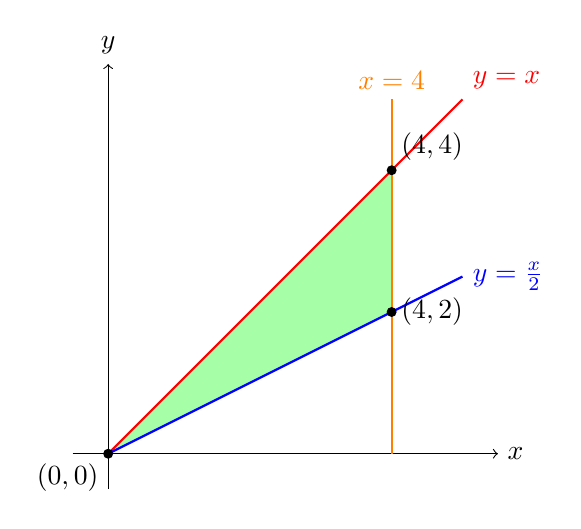
\begin{tikzpicture}[scale=0.9]

    % Axes
    \draw[->] (-0.5,0) -- (5.5,0) node[right] {$x$};
    \draw[->] (0,-0.5) -- (0,5.5) node[above] {$y$};

    % Shaded region
    \fill[green!35] (0,0) -- (4,4) -- (4,2) -- cycle;

    % Boundary lines
    \draw[thick, red] (0,0) -- (5,5) node[above right] {$y=x$};
    \draw[thick, blue] (0,0) -- (5,2.5) node[right] {$y=\frac{x}{2}$};
    \draw[thick, orange] (4,0) -- (4,5) node[above] {$x=4$};

    % Key points
    \fill (0,0) circle (2pt) node[below left] {$(0,0)$};
    \fill (4,4) circle (2pt) node[above right] {$(4,4)$};
    \fill (4,2) circle (2pt) node[right] {$(4,2)$};

\end{tikzpicture}
\end{center}

    \begin{align*}
        \iint_D (x^3+y^3)dxdy&= \int_0^4\left(\int_{y=\frac{x}{2}}^{y=x}(x^3+y^3)dy\right)dx\\
        &= \int_0^4 \left.\left(x^3y+\frac{y^4}{4}\right)\right|_{y=\frac{x}{2}}^{y=x}dx
    \end{align*}
\end{example}

\begin{example}
Find the area of the region bounded by the curves
\[
y=1, \qquad x=y^2, \qquad x+2y+1=0.
\]

\textbf{Solution.}

The line $x+2y+1=0$ can be written as $x=-2y-1$. For \(-1 \le y \le 1\), the left boundary is
\[
x=-2y-1,
\]

and the right boundary is
\[
x=y^2.
\]

Therefore, the required area is
\begin{align*}
A&=\int_{-1}^{1}\left[y^2-(-2y-1)\right]\,dy\\
&=\int_{-1}^{1}(y^2+2y+1)\,dy\\
&=\int_{-1}^{1}(y+1)^2\,dy\\
&=\int_{-1}^{1}(y+1)^2\,dy\\
&=\left[\frac{(y+1)^3}{3}\right]_{-1}^{1}\\
&=\boxed{\frac{8}{3}}  
\end{align*}
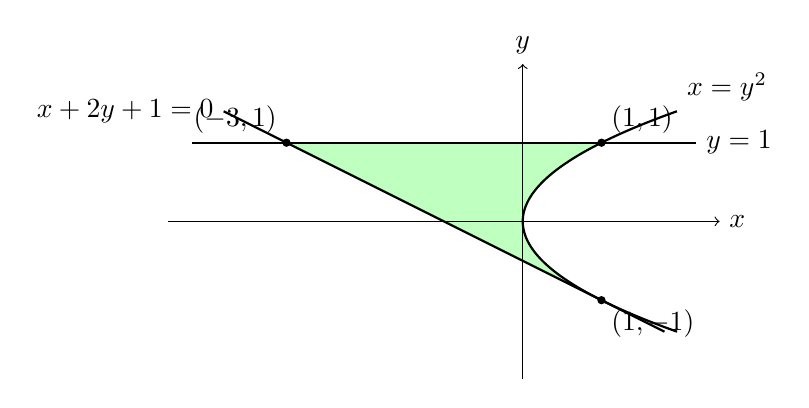
\begin{tikzpicture}[scale=1]

    % Shaded bounded region
    \fill[green!25]
        plot[domain=-1:1,samples=100,smooth,variable=\y]
            ({\y*\y},{\y})
        --
        plot[domain=1:-1,samples=100,smooth,variable=\y]
            ({-2*\y-1},{\y})
        -- cycle;

    % Axes
    \draw[->] (-4.5,0) -- (2.5,0) node[right] {$x$};
    \draw[->] (0,-2) -- (0,2) node[above] {$y$};

    % Curves
    \draw[thick] (-4.2,1) -- (2.2,1) node[right] {$y=1$};

    \draw[thick,domain=-1.4:1.4,samples=100,smooth,variable=\y]
        plot ({\y*\y},{\y}) node[above right] {$x=y^2$};

    \draw[thick,domain=-1.4:1.4,samples=100,smooth,variable=\y]
        plot ({-2*\y-1},{\y}) node[left] {$x+2y+1=0$};

    % Intersection points
    \fill (-3,1) circle (1.5pt) node[above left] {$(-3,1)$};
    \fill (1,1) circle (1.5pt) node[above right] {$(1,1)$};
    \fill (1,-1) circle (1.5pt) node[below right] {$(1,-1)$};

\end{tikzpicture}
\end{example}


